\chapter{SV Detection in Single Cells}
\label{sec:mosaicatcher}

\ashley, \jan, \marschall, \david, \maryam, \venla

\section{Structural variants in the context of somatic mosaicism}
\label{sec:mosaic_mosaicism}



\section{\textsc{Mosaicatcher}: A novel approach for comprehensive SV detection in single-cell Strand-seq data}
\label{sec:mosaic_mc}


\afterpage{%
    \clearpage%
    \ifodd\value{page} \expandafter\afterpage \fi {%
    \begin{figure}[t!]                                             % cell BM160815_WT_007p1 from BM160815_WT.200000.pdf
        \captionsetup{type=figure}
        \figcap{ss_library}{Example of a single cell Strand-seq library}{
            Here, a single cell Strand-seq library of an \rpe-I wild type cell
            line is displayed using the plot function of \mc.
            Each vertical panel shows binned read counts of one chromosome, with
            the Watson strand on the left, in orange, and the Crick strand on
            the right in blue. In the cell shown here, each 200~kb-bin contains
            a median of 76 total reads, which is depicted by the
            dotted lines. Some regions, e.g. the centromere of chromosome 1 or
            the sub-telomeric regions of chromosomes 13--15 are not coverded by
            reads because of mappability issues; these bins are excluded from
            further analyses. The estimated strand inheritance state of each bin
            is color-coded in the background: blue for CC, orange for WW and yellow
            for WC. Chromosomes 5 and 11 carry \acp{sce}, which are visible by a
            change in the strand inheritance state that continues to the end of
            the chromosomes.}%
        \vspace{-3cm}%
        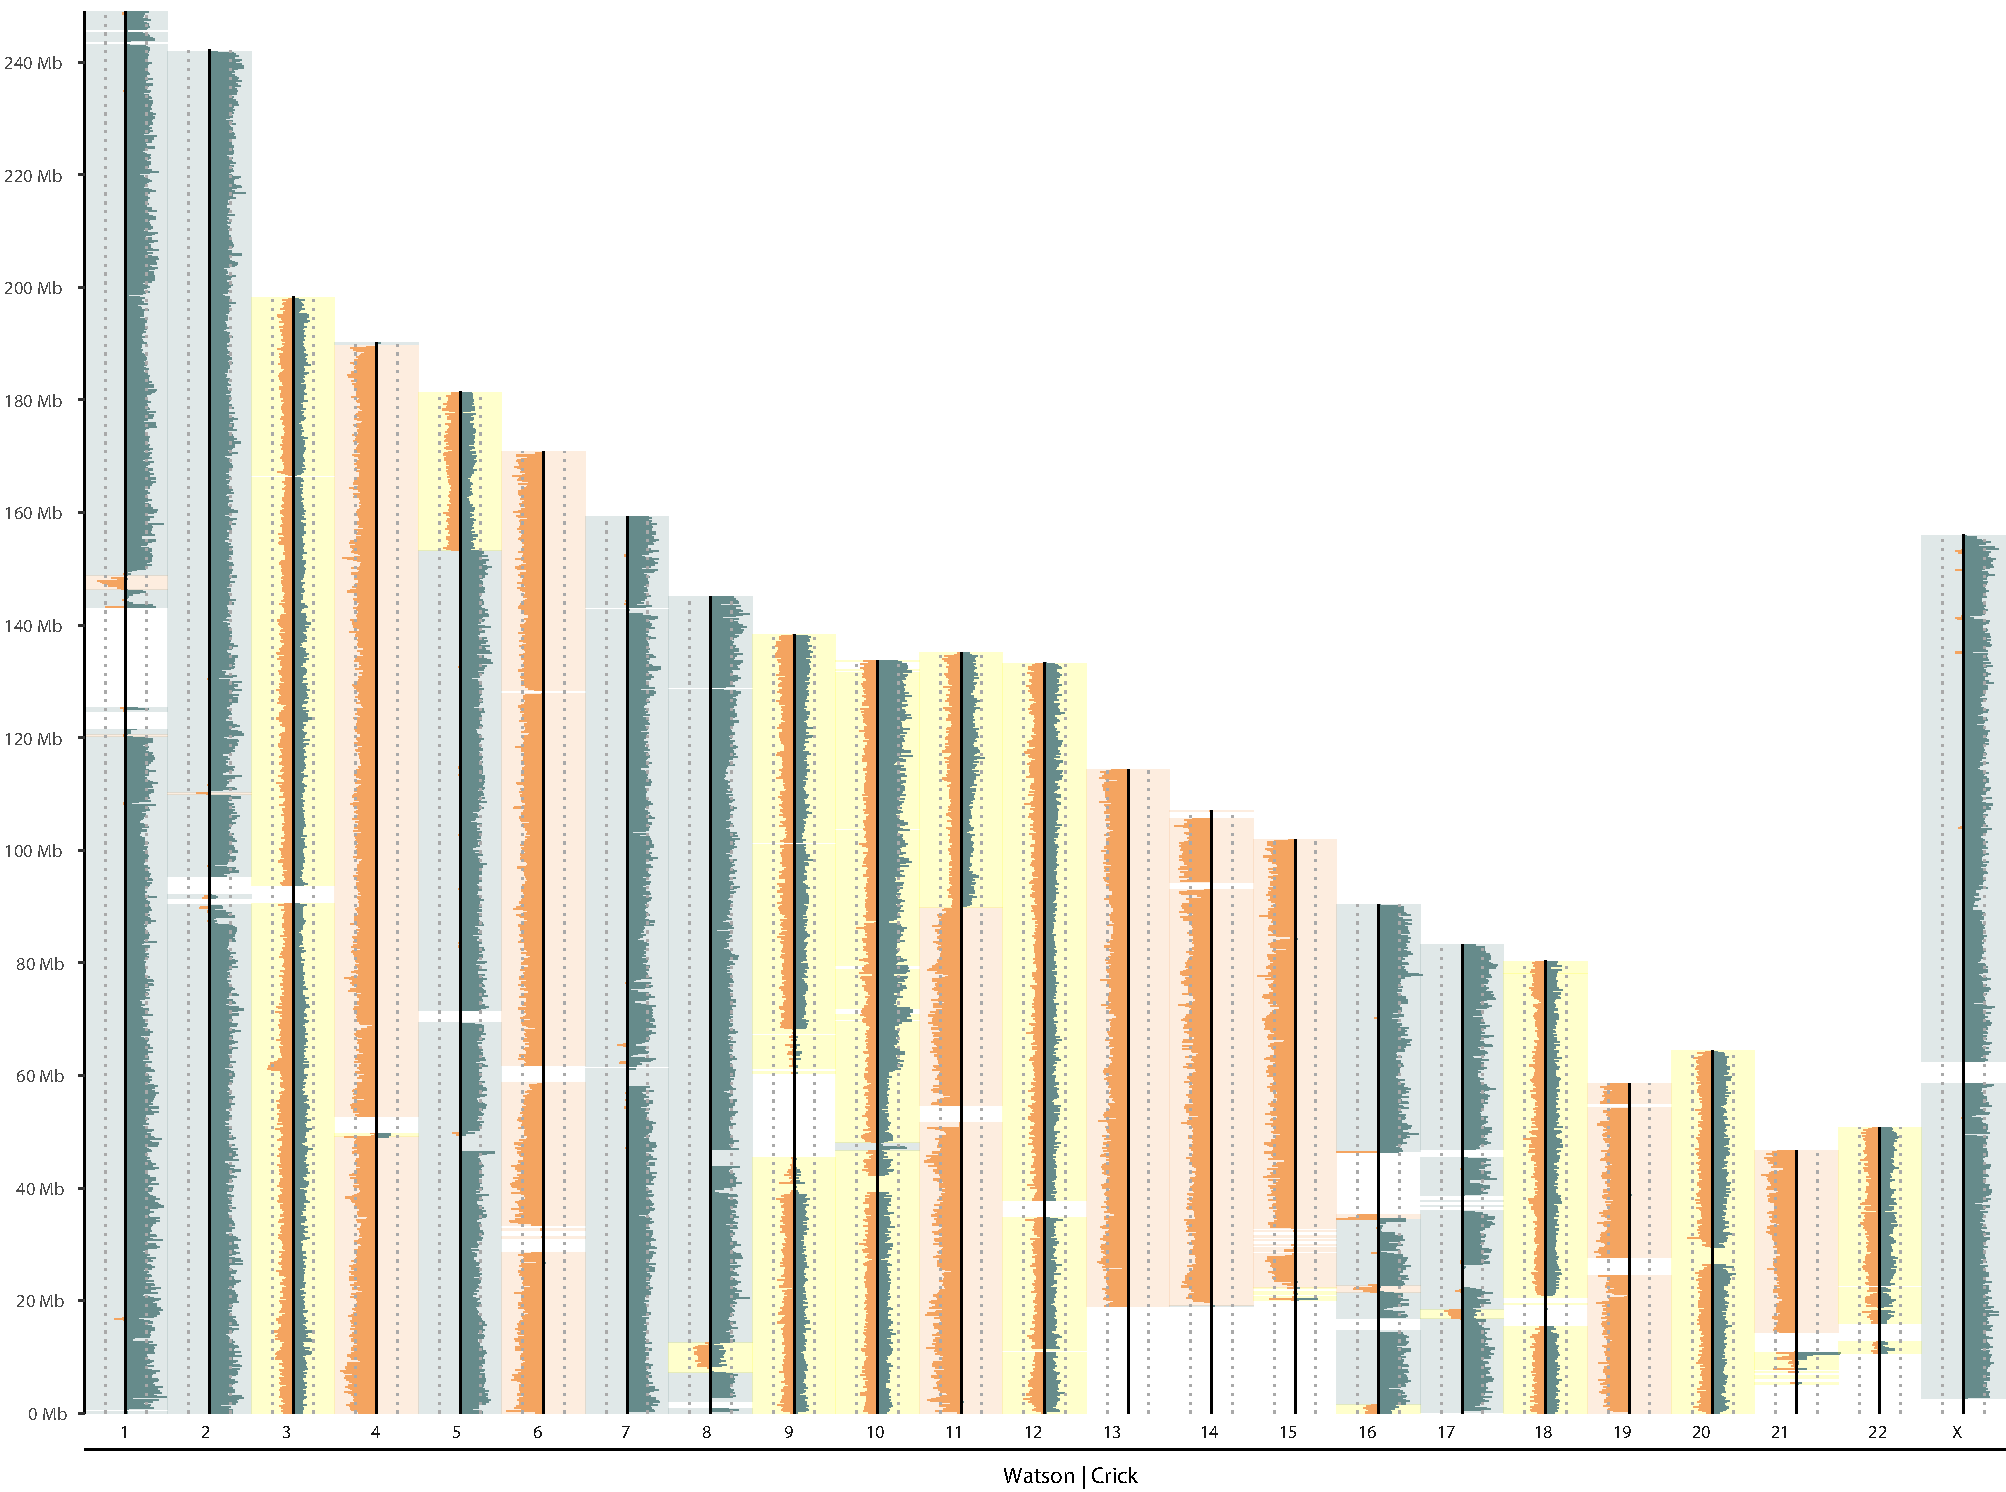
\includegraphics[width=\textplusmargin,inner]{ss_lib_rpewt.pdf}
    \end{figure}
    }}



\subsection{Three signals within Strand-seq data are distinctive of SVs}
\label{sec:mosaic_concept}



\subsection{Automatd SV detecting}
\label{sec:mosaic_method}



\subsection{Revealing potential SV breakpoints via multivariate total variation denoising}
\label{sec:mosaic_segmentation}


\FloatBarrier
\section{Simulation of Strand-seq data to explore the limits of \textsc{Mosaicatcher}}
\label{sec:mosaic_simul}

\subsection{Development of a versatile simulation framework}

\subsection{Assessing the performance of the segmentation algorithm}

\section{Conclusions and outlook}
\label{sec:mosaic_conclusion}


